\section{Methodologies and Experiments}
\begin{figure}
    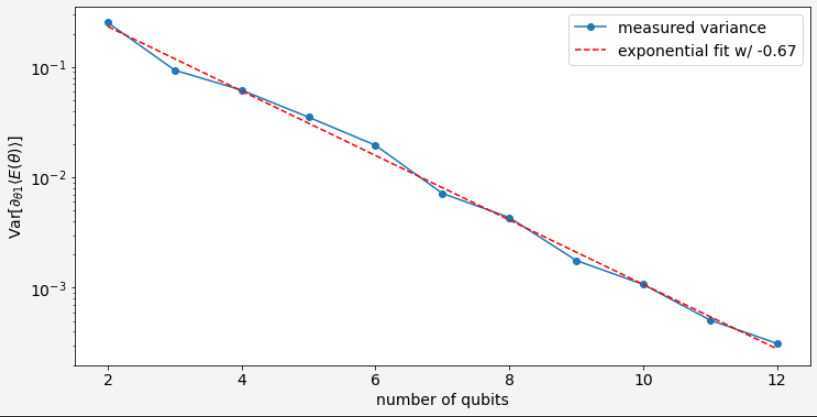
\includegraphics[width=\textwidth]{./ResearchDesign/Appendices/VarianceShrinking.png}
    \caption{
        An example of Barren Plateaus phenomenon occurs to a QNN model. 
        The variance of the gradient shrinking \textit{exponentially} with the number of qubits. 
        Barren Plateaus phenomenon prevents optimization algorithms to navigate the cost function landscape efficiently.
    }
    \label{Variance Shrinking demo}
\end{figure}

Cerezo et al. has pointed out that Barren Plateaus is cost function dependent \cite{cerezoCostFunctionDependent2021}, which implies that the only way to fully eliminate Barren Plateaus is to use a local cost function with a shallow circuit.
However, there are still other approaches to mitigate the phenomenon without using the local cost function.
Skolik et al. and Liu et al. \cite{skolikLayerwiseLearningQuantum2021, liuParameterInitializationMethod2021} suggest that we can initiate the starting parameters away from plateaus to guarantee the trainability from the first steps.
In this section, we design the methodologies to conduct the experiment to answer the research question.

\subsection{Research Type Overview}
We have examined the three theories \cite{cerezoCostFunctionDependent2021, liuParameterInitializationMethod2021, skolikLayerwiseLearningQuantum2021} in the literature review, and it is suggested that an empirical experiment can be conducted to compare the three.
Consequently, the result of this experiment is a table that record the performance of the three methods in some criteria.

The main advantage of experimentation methodology is that we can fully control the experiment environment and its subjects, objects, etc.
In this case, these are the factors that leads to Barren Plateaus, the configuration for the QNN ansatz, and the three implementation of theories on the QNN ansatz.
We elaborate the research process in later sections.

\subsection{Research Activities}
\label{Research Activities section}
\textbf{In the first phase, we create a QNN model to reproduce the Barren Plateaus.} 
We can use Qiskit \cite{Qiskit} to construct the ansatz, and most importantly, it provides a quantum emulator that capable of simulate up to 32 qubits.
The literature review had pointed out that the two factors causing Barren Plateaus are the \textit{ansatz depth, large number of qubits} and the \textit{randomised starting parameters}, so we configure the ansatz to have such characteristics in a quantum simulator.
Then we calculate the variance of the gradient, and expect the variance is shrinking \textit{exponentially} with the number of qubits (see Figure \ref{Variance Shrinking demo}).
The result will be a QNN ansatz with the depth and number of qubit enough to produce the Barren Plateaus.

\textbf{In the second phase, we implement the three approaches}.
With the QNN ansatz from the first step we can implement the three methods as discussed in the literature review.
The Qiskit framework also support the mutation for the ansatz object, such as the number of qubit to measure, the depth of ansatz (repetition) and the starting parameters.
We will track the variances of the gradient for each method to identify if the model has mitigated the Barren Plateaus phenomenon.

The results of the research activities is discussed in Subsection \ref{Data Collecting Section}

\subsubsection{Criteria}
\label{Criteria section}
The data can be compared with these criteria:
\begin{itemize}
    \item How good the solution is;
    \item The size of the circuit;
    \item The size of the qubit registry;
    \item The time required to execute the circuit;
    \item The complexity of the algorithms.
\end{itemize}

\subsubsection{Hypothesis}
The experiment activities are formalized into two hypotheses:
\begin{itemize}
    \item \textbf{Null}: The three methods have the same performance according to the criteria, or the different is insignificant;
    \item \textbf{Alternative}: The three methods performance differ when reflect the result against the criteria.
\end{itemize}

\subsection{Data Collecting Method}
\label{Data Collecting Section}
Here we discuss our method to collect the data from the experiment.

The output of the first phase is a Qiskit ansatz object that contains the number of qubits, the depth of the circuit (rep), and the parameter is configured randomly.
Moreover, the ansatz object in Qiskit is mutable, which means that we can modify the ansatz properties in the second phase.

For the second phase, we need to record three different outputs of the three methods accordingly, with the criteria as defined in Subsection \ref{Criteria section}.
The result is a table with the criteria in the Subsection \ref{Criteria section}.
With this data, we can decide whether to reject the null hypothesis or not.

Finally, we summarize the table to present the findings.

\subsection{Resources}
Most of our required resources are open-sources:
\begin{itemize}
    \item Python 3.6+: \url{https://www.python.org/downloads/}
    \item Anaconda: \url{https://www.anaconda.com/products/distribution}
    \item Jupyter Notebook: \url{https://jupyter.org/}
    \item Qiskit: \url{https://qiskit.org/}
    \item IBM Quantum: \url{https://quantum-computing.ibm.com/}
\end{itemize}

To prepare the quantum emulator in local machine, we first install Python and Anaconda for programming language support, Jupyter Notebook as code editing tool.
Then we follow the official instruction from Qiskit \cite{Qiskit} to install the necessary packages.
We can start working with Qiskit in a Jupyter Notebook file.

The other option is to use the provided Python kernel with Qiskit provided by IBM Quantum.

To construct the ansatz as discussed in Section \ref{Research Activities section}, we can use the "Real Amplitudes" circuit provided by Qiskit.


\subsection{Success Condition}
The experiment will be concluded when these conditions are met:
\begin{itemize}
    \item We have a QNN ansatz that possesses Barren Plateaus;
    \item The three methods are implemented;
    \item The data from the three methods are evaluated against the criteria;
    \item We have identified when to use which method to counter Barren Plateaus.
\end{itemize}